\section{Esercizio 23}
\textit{\textbf{Descrizione:}  Sapendo che}

\begin{equation}
  \begin{aligned}
      & I(x) =\int_{0}^{atan(30)}(1+tan^{2}(x))dx = 30
  \end{aligned}
\end{equation}

\noindent\textit{tabulare il numero dei punti richiesti dalle formule composite dei trapezi e di Simpson per approssimare $I(f)$ con tolleranze $tol=10^{-i}$, con $i = 2,\cdots,8$}
\\~\\
\noindent\emph{Soluzione: }\newline
per prima cosa \'e stato necessario effettuare una modifica al metodo dei trapezi adattivo e al metodo di Simpson adattivo per fare in modo che ritornassero \newline
il numero di punti\\~\\

\lstinputlisting{resources/trapadcount.m}\newpage
\lstinputlisting{resources/simpadcount.m}\newpage
poi si \'e eseguito il seguente script per visualizzare i risultati\newline
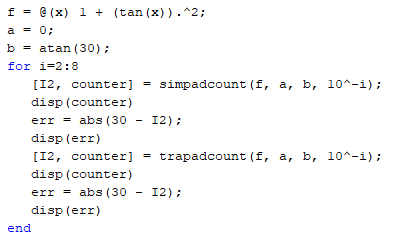
\includegraphics[width=1\linewidth]{img/ex23}\\~\\
ottenendo cos\'i i risultati della seguente tabella\\~\\
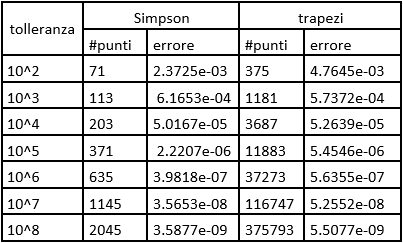
\includegraphics[width=1.3\linewidth]{img/tabella23}
